\documentclass[12pt, letter]{exam}
\usepackage[utf8]{inputenc}
\usepackage[T1]{fontenc}
\usepackage[spanish]{babel}
\usepackage{amsmath}
\usepackage{amsthm}
\usepackage{physics}
\usepackage{tikz}
\usepackage{float}
\usepackage{siunitx}
\usepackage{multicol}
\usepackage[left=2.00cm, right=2.00cm, top=2.00cm, 
     bottom=2.00cm]{geometry}
\usepackage{pdfpages}

% \renewcommand{\questionlabel}{\thequestion}
\decimalpoint

\setlength{\belowdisplayskip}{-0.5pt}

\usepackage{tasks}
\settasks{
    label=\Alph*), 
    label-align=left,
    item-indent={20pt}, 
    column-sep={4pt},
    label-width={16pt},
}

\sisetup{per-mode=symbol}
\footer{}{\thepage}{}

\begin{document}
\includepdf[pages={1}]{Caratula_Examen_Parcial_PU_Fisica_4_03.pdf}

\newpage
% 4 ejercicios de ejecución
\begin{questions}
    \question \textbf{(5 puntos)} A continuación se te presenta la definición de 5 conceptos, la palabra faltante está en la parte inferior, relaciona cada definición con la palabra.
    \begin{parts}
        \part \rule{2cm}{0.3mm} es la distancia entre la elongación máxima y su posición de equilibrio.
        \part \rule{2cm}{0.3mm} es la distancia que separa dos puntos equivalentes consecutivos de la onda.
        \part \rule{2cm}{0.3mm} es el tiempo que se necesita para hacer una oscilación completa.
        \part \rule{2cm}{0.3mm} es el número de oscilaciones o vibraciones que realiza la onda por unidad de tiempo.
        \part \rule{1.5cm}{0.3mm} es el recorrido de la onda desde un punto hasta el siguiente punto equivalente.
    \end{parts}
    
    \begin{center}
        I) Ciclo, \hspace{0.2cm} II) Cresta, \hspace{0.2cm} III) Longitud de onda, \hspace{0.2cm} IV) Periodo, \\[0.5em] V) Amplitud, \hspace{0.2cm} VI) Frecuencia, \hspace{0.2cm} VII) Elongación
    \end{center}
    {
    \renewcommand{\thepartno}{\Alph{partno}}
    \renewcommand{\partlabel}{\thepartno)}
    \begin{parts}
        \part a) - II), b) - III), c) - V), d) - VI) e) - I)
        \part a) - V), b) - III), c) - IV), d) - VI) e) - I)
        \part a) - IV), b) - V), c) - I), d) - VI) e) - II)
        \part a) - IV), b) - V), c) - II), d) - III) e) - I)
    \end{parts}}
    Con la siguiente figura se muestra una onda transversal cuya frecuencia es de \SI{12}{\hertz}, responde las preguntas \textbf{\ref{completa_grafica_01}}, \textbf{\ref{completa_grafica_02}}, \textbf{\ref{completa_grafica_03}}, \textbf{\ref{completa_grafica_04}}.
    \begin{figure}[H]
        \centering
        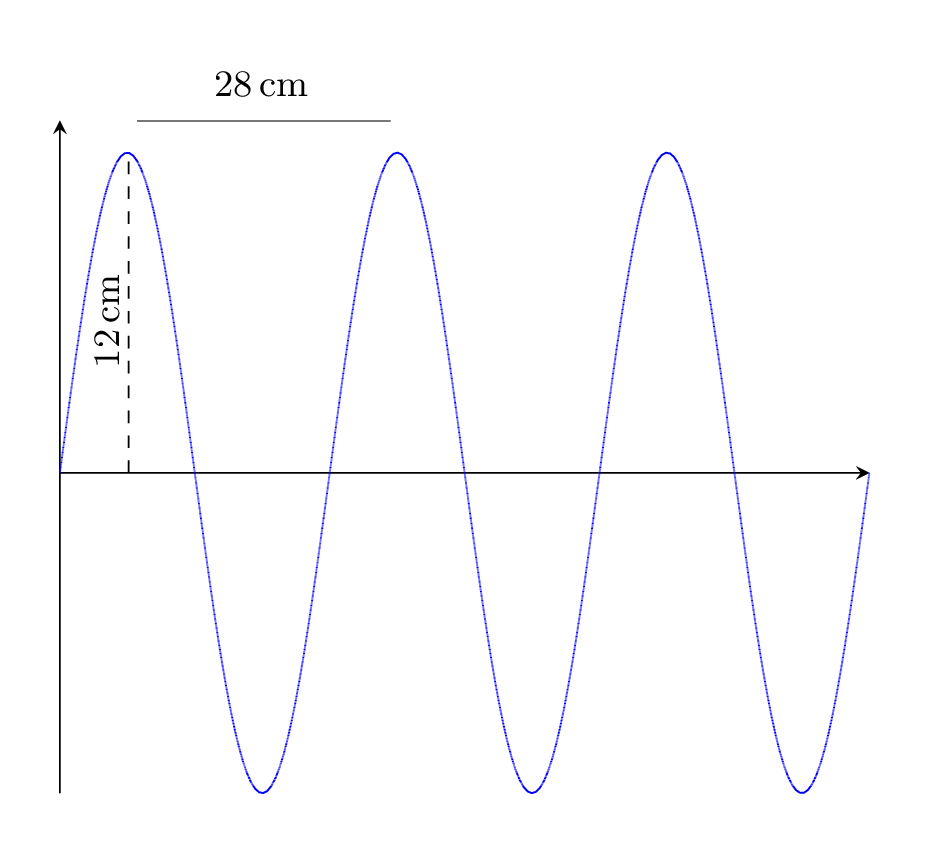
\includegraphics[scale=0.3]{Imagenes/Grafica_Onda_Examen_01.png}
    \end{figure}
    \question \label{completa_grafica_01} ¿Cuál es la amplitud?
    \begin{tasks}(4)
        \task \SI{8}{\centi\meter}
        \task \SI{10}{\centi\meter}
        \task \SI{12}{\centi\meter}
        \task \SI{14}{\centi\meter}
    \end{tasks}
    \question \label{completa_grafica_02} ¿Cuál es la longitud de onda?
    \begin{tasks}(4)
        \task \SI{28}{\centi\meter}
        \task \SI{30}{\centi\meter}
        \task \SI{32}{\centi\meter}
        \task \SI{34}{\centi\meter}
    \end{tasks}
    \question \label{completa_grafica_03} ¿Cuál es el periodo?
    \begin{tasks}(4)
        \task \SI{0.83}{\second}
        \task \SI{8.33d-3}{\second}
        \task \SI{83.3d-3}{\second}
        \task \SI{103.3d-3}{\second}
    \end{tasks}
    \question \label{completa_grafica_04} ¿Cuál es la rapidez?
    \begin{tasks}(4)
        \task \SI{0.336}{\meter\per\second}
        \task \SI{3.36}{\meter\per\second}
        \task \SI{33.36}{\meter\per\second}
        \task \SI{333.6}{\meter\per\second}
    \end{tasks}
    En las preguntas \textbf{\ref{completa_01}}, \textbf{\ref{completa_02}}, \textbf{\ref{completa_03}}, \textbf{\ref{completa_04}}, \textbf{\ref{completa_05}} completa la definición con uno de las palabras que se señalan en las opciones.
    \question \label{completa_01} Se definen las ondas longitudinales a aquellas que se generan cuando las partículas del medio material vibra de manera \rule{2cm}{0.3mm} a la dirección de propagación de la onda.
    \begin{tasks}(4)
        \task Uniforme
        \task Perpendicular
        \task Reflejante
        \task Paralela
    \end{tasks}
    \question \label{completa_02} Cuando mencionamos que este fenómeno se produce cuando las ondas encuentran un obstáculo en su camino y lo rodean, hablamos de la \rule{2cm}{0.3mm} de ondas.
    \begin{tasks}(4)
        \task Reverberancia
        \task Reflexión
        \task Difracción
        \task Refracción
    \end{tasks}
    \question \label{completa_03} La \rule{2cm}{0.3mm} se produce cuando un tren de ondas encuentra un obstáculo que les impide propagarse.
    \begin{tasks}(4)
        \task Reflexión
        \task Resonancia
        \task Refracción
        \task Difracción
    \end{tasks}
    \question \label{completa_04} El fenómeno de la \rule{2cm}{0.3mm} se presenta cuando las ondas pasan de un medio a otro de distinta densidad.
    \begin{tasks}(4)
        \task Eco
        \task Reflexión
        \task Difracción
        \task Refracción
    \end{tasks}
    \question \label{completa_05} Cuando la vibración de un cuerpo hace vibrar a otro con la misma frecuencia, estamos definiendo a la \rule{2cm}{0.3mm}
    \begin{tasks}(4)
        \task Reflexión
        \task Difracción
        \task Refracción
        \task Resonancia
    \end{tasks}
    \question \textbf{Problema de ejecución.} En una cuerda tensa se producen ondas con una frecuencia de \SI{240}{\hertz}, a una velocidad de propagación cuya magnitud es de \SI{150}{\meter\per\second}. ¿Qué longitud de onda tienen?
     \begin{tasks}(4)
        \task \SI{0.625}{\meter}
        \task \SI{0.855}{\meter}
        \task \SI{1.920}{\meter}
        \task \SI{1.102}{\meter}
    \end{tasks}
     \question \textbf{Problema de ejecución.} Determinar cuál es el periodo de las ondas producidas en una cuerda de violín si la velocidad de propagación tiene una magnitud de \SI{220}{\meter\per\second} y su longitud de onda es de $\lambda = \SI{0.2}{\meter}$.
     \begin{tasks}(4)
        \task \SI{9.09d-2}{\second}
        \task \SI{9.09d-3}{\second}
        \task \SI{9.09d-4}{\second}
        \task \SI{9.09d-5}{\second}
     \end{tasks}
     \question \textbf{Problema de ejecución.} Una fuente sonora produce un sonido con una frecuencia de \SI{750}{\hertz}, calcula su longitud de onda en el agua, considera que la magnitud de la velocidad del sonido en el agua es de \SI{1435}{\meter\per\second}.
     \begin{tasks}(4)
        \task \SI{1.813}{\meter}
        \task \SI{1.913}{\meter}
        \task \SI{2.856}{\meter}
        \task \SI{3.102}{\meter}
    \end{tasks}
    \question \textbf{Problema de ejecución.} ¿Cuál es la intensidad de un sonido de \SI{40}{\dB}?
    \begin{tasks}(4)
        \task \SI{1d-8}{\watt\per\square\meter}
        \task \SI{1d-9}{\watt\per\square\meter}
        \task \SI{1d-10}{\watt\per\square\meter}
        \task \SI{1d-11}{\watt\per\square\meter}
    \end{tasks}
    \question Ángulo con el cual la diferencia de fase de dos ondas en interferencia destructiva, hace que la suma vectorial de las amplitudes sea cero.
    \begin{tasks}(4)
        \task \ang{0}
        \task \ang{90}
        \task \ang{180}
        \task \ang{270}
    \end{tasks}
    \question Sabemos que el efecto Doppler se refiere al cambio aparente en la frecuencia de una fuente
    de sonido cuando hay un movimiento de la fuente y del oyente, el movimiento entre ambos es de tipo:
    \begin{tasks}(4)
        \task Relativo
        \task Creciente
        \task Absoluto
        \task Decreciente
    \end{tasks}

\end{questions}

\newpage

\textbf{\huge{Formulario.}}
\begin{table}[H]
    \centering
    \setlength{\tabcolsep}{40pt}
    \renewcommand{\arraystretch}{2.5}
    \begin{tabular}{c  c}
            $v = \lambda \, f$ & $T = \dfrac{1}{f}$ \\
		    $\dfrac{\lambda_{1}}{\lambda_{2}} = \dfrac{v_{1}}{v_{2}}$ & $B = 10 \, \log \left( \dfrac{I}{I_{0}} \right)$ \\
            $I_{0} = \SI{1d-12}{\watt\per\square\meter}$ & $\lambda = \dfrac{2 \, L}{n}$ \\
            $f_{0} = f_{s} \, \dfrac{V + v_{0}}{V - v_{s}}$ &  \\
\end{tabular}
\end{table}

\end{document}